\documentclass[12pt,a4paper, spanish]{report}
\usepackage[spanish]{babel}
\usepackage[latin1]{inputenc}  % Ambos para solucin de asuntos de idioma
\usepackage[T1]{fontenc}
\usepackage{tocbibind}  % Bibliografa en el indice
\usepackage{titlesec}  % Posibilidad de editar los formatos de chapter y section
%\usepackage{times}  % Fuente de letras
\usepackage{amsmath,amssymb,mathrsfs,mathptmx}  % Matemticas varias
\usepackage{hyperref} % Para escribir URLs
\usepackage[vlined,ruled]{algorithm2e}
\usepackage{hyperref}

% --- Arreglos varios para la inclusion de imgenes
%\usepackage[pdftex]{graphicx}
%\usepackage[dvips]{graphicx}
\usepackage{graphicx}
\usepackage{epsfig}
%\usepackage{epstopdf}


\usepackage{float}
\usepackage{subfigure}
%\usepackage{subfig}
\usepackage{wrapfig}
\usepackage[usenames,dvipsnames]{color}
\DeclareGraphicsExtensions{.png,.jpg,.pdf,.mps,.gif,.bmp, .eps}


\usepackage{multirow}
\usepackage{multicol}
\usepackage{tabulary}
\usepackage[table]{xcolor}
\usepackage{color}
\usepackage{listings}
%\usepackage{subfloat}
\usepackage{tikz}

\setcounter{secnumdepth}{3}
\setcounter{tocdepth}{3}


% --- Para las dimensiones de los mrgenes etc
\frenchspacing \addtolength{\hoffset}{-1.5cm}
\addtolength{\textwidth}{3cm} \addtolength{\voffset}{-2.5cm}
\addtolength{\textheight}{4cm}
% --- Para el encabezado
\usepackage{fancyhdr}
\fancyhead[R]{2012}\fancyhead[L]{enCuadro} \fancyfoot[C]{\thepage}
\pagestyle{fancy}

% --- Formato de la etiqueta Chapter
%\newcommand{\bigrule}{\titlerule[0.5mm]}
%\titleformat{\chapter}[display]{\bfseries\Huge}
%{\Large\chaptertitlename\ \Large\thechapter}
%{0mm} {\filleft} [\vspace{0.5mm} \bigrule]

\titleformat{\chapter}[display]
{\normalfont\Large\filcenter}
{\titlerule[1pt]%
\vspace{1pt}%
\titlerule
\vspace{1pc}%
\LARGE\MakeUppercase{\chaptertitlename} \thechapter}
{1pc}
{\titlerule
\vspace{1pc}%
\Huge}

%-------------------------

\begin{document}
% Esto es para que se muestren todas las referencias aunque no se citen:
\nocite{*}

\renewcommand{\tablename}{Tabla}
\renewcommand{\theenumi}{\Roman{enumi}}
\renewcommand{\labelenumi}{[\textbf{\theenumi}]}
\renewcommand{\thefootnote}{\arabic{footnote}}
% --- Modificacin de entornos enumerate
\renewcommand{\theenumi}{\roman{enumi}}
\renewcommand{\labelenumi}{\theenumi)}
% --- Modificacin de entornos enumerate

% --- Para hacer highlights
\newcommand{\highlAmarillo}[1]{\colorbox{yellow}{#1}}
\newcommand{\highlVerde}[1]{\colorbox{green}{#1}}
\newcommand{\highlRojo}[1]{\colorbox{red}{#1}}

%--- Para indicar la norma de algo
\providecommand{\norm}[1]{\lVert#1\rVert}

\begin{titlepage}

\vskip2.5cm
\begin{center}
\begin{tabular}{p{1cm} p{11cm}  p{1cm}}
 &
\large{
\begin{center}
\sc Proyecto de fin de estudios \\
\sc en la carrera Ingenier�a El�ctrica\\
\end{center}
} &
\end{tabular}
\end{center}

%\begin{picture}(0,0)
%\put(-35,20){\includegraphics[width=5cm]{Imagenes/logo_udelar.eps}}
%\end{picture}

%\begin{picture}(0,0)
%\put(338,35){\includegraphics[width=5cm]{Imagenes/logo_udelar.eps}}
%\end{picture}

\vskip3cm

\begin{center}
\Huge {\textbf{encuadro}}\\
\Large {Aplicaci�n de realidad aumentada y navegaci�n para museos sobre dispositivos m�viles}
\end{center}

\vskip2cm

\begin{center}
\Large {\sc \textbf{Documentaci�n Final}}\\
\Large {\sc \textbf{A\~no 2012}}\\
\end{center}

\vskip2cm

%\begin{center}
%\Large {\textbf{CubeSatET} es parte del \textbf{Proyecto LAI}}\\
%\end{center}

\vskip3cm

\begin{flushright}
\begin{tabular}{r l}
\large{\underline{\bf Tutor:}}\vspace{0.2cm}\\
\large{\textbf{Juan Cardelino}}\\
\end{tabular}
\end{flushright}

\vskip1cm

\begin{flushright}
\begin{tabular}{r l}
\large{\underline{\bf Integrantes:}}\vspace{0.2cm}\\
\large{\textbf{Juan Braun}}\\
juanibraun@gmail.com\\
\large{\textbf{Mart�n Etchart}}\\
mrtn.etchart@gmail.com\\
\large{\textbf{Pablo Flores}}\\
pablofloresguridi@gmail.com\\
\large{\textbf{Mauricio Gonz�lez}}\\
mgonzaleznappa@gmail.com\\
\end{tabular}
\end{flushright}


\end{titlepage}

\tableofcontents

\chapter{\textit{Rendering} en iOS: ISGL3D}
% v5.0: Corregida por el tribunal.
\label{chap: render}
\section{Introducci�n}
\textit{Rendering} es un t�rmino en ingl�s que denota el proceso de generar una imagen 2D a partir de un modelo digital 3D o un conjunto de ellos, a los que se les llama ``escena''. Puede ser comparado con tomar una foto o filmar una escena en la vida real, en donde se tiene una c�mara, luces y actores u objetos. Cada uno de estos componentes tiene su equivalente digital cuando se hace un \textit{render}. Afortunadamente, existen varias herramientas de \textit{rendering}, tambi�n llamadas ``motores de juego 3D'', para plataformas m�viles, en especial que funcionen sobre iOS. Algunas de ellas son Unity 3D, ISGL3D, Cocos3D, Open GL ES y ShiVa3D. A continuaci�n ser�n comentadas tan s�lo las consideradas durante el presente proyecto por ser populares y gratuitas.\\

La primera en ser tomada en cuenta fue ``Open Graphics Library Embedded Systems'' (Open GL ES), que es un subconjunto de las herramientas de gr�ficos 3D de Open GL. Fue dise\~nada para ser utilizada sobre sistemas embebidos (dispositivos m�viles, consolas de video juegos, etc.); Open GL es el est�ndar m�s ampliamente usado alrededor del mundo para la creaci�n de gr�ficos 2D y 3D, es gratis y multiplataforma. Como la programaci�n en Open GL y en particular en Open GL ES es de muy bajo nivel y por lo tanto bastante complicada, se opt� por investigar otras herramientas. Se descubri� entonces ISGL3D \cite{isgl3d12} un \textit{framework} escrito en Objective-C que trabaja sobre Open GL ES y que busca facilitar la tarea del programador al momento de crear y manipular escenas 3D mediante una ``\textit{Application Program Interface}'' (API) sencilla e intuitiva. Es un proyecto gratis y en c�digo abierto. Luego de algunas semanas de trabajo con la herramienta e importantes avances desde el punto de vista del manejo de la misma se descubri� la existencia de otro \textit{framework} de id�nticas caracter�sticas llamado ``Cocos3D''. Cocos3D es una extensi�n de ``Cocos2D'', una herramienta para la generaci�n de gr�ficos 2D,  muy popular entre los desarrolladores de aplicaciones para iOS. Como no se identificaron diferencias significativas entre ISGL3D y Cocos3D, se prioriz� el tiempo dedicado a ISGL3D y se decidi� continuar trabajando de forma inalterada. Al d�a de hoy, sobre el final del proyecto, se cree que si bien t�cnicamente ambos \textit{frameworks} son muy buenos y a la vez similares entre s�, ISGL3D parece estar algo m�s avanzado en cuanto a su desarrollo. Sin embargo debido a la gran popularidad de Cocos2D, Cocos3D ha heredado muchos usuarios y cuenta con una comunidad mucho m�s activa, lo que facilita mucho su uso y hace pensar que en un futuro cercano resulte en un \textit{framework} m�s desarrollado.\\

En este cap�tulo se comentar�n algunas caracter�sticas y conceptos de ISGL3D que fueron importantes para el proyecto;  por detalles de algunos temas en particular referirse a la referencia de la ya mencionada API en: \url{www.isgl3d.com/resources/api}.  Adem�s se trazar� una hoja de ruta para todo aquel que quiera iniciarse en el manejo de la herramienta.\\


\section{Conceptos b�sicos de ISGL3D}
ISGL3D es un motor de juegos 3D para \textit{iPad}, \textit{iPhone} y \textit{iPod touch} escrito en \textit{Objective-C}, que sirve para crear escenas y \textit{renderizarlas} de forma sencilla. Es un proyecto en c�digo abierto y gratis. En su sitio web oficial: \url{www.isgl3d.com}, se puede descargar su c�digo, y de forma sencilla ISGL3D puede ser agregado como un complemento de \textit{Xcode}. Adem�s se pueden encontrar tutoriales, detalles de su API y un acceso a un grupo de \textit{Google} donde la comunidad pregunta y responde dudas propias y ajenas. Una buena manera de iniciarse en manejo de la herramienta es siguiendo los tutoriales en: \url{www.isgl3d.com/resources/tutorials}; al menos este fue el camino elegido por el grupo. Los tutoriales son 6, y abarcan distintos t�picos:
\begin{itemize}
\item \textbf{Tutorial 0:} primer paso en el creado de una aplicaci�n ISGL3D. Cubre algunos conceptos b�sicos y muestra c�mo integrar la herramienta a \textit{Xcode}.
\item \textbf{Tutorial 1:} mustra c�mo crear una escena bien simple, con tan s�lo un cubo en rotaci�n continua.
\item \textbf{Tutorial 2:} ense\~na c�mo agregar luz a una escena. Se ven las distintas fuentes de luz que existen en el \textit{framework}.
\item \textbf{Tutorial 3:} se ve c�mo hacer para mapear texturas en los objetos 3D con el objetivo de hacerlos m�s realistas.
\item \textbf{Tutorial 4:} muestra c�mo crear interacci�n entre el usuario y los distintos objetos ISGL3D, cuando este los toca a trav�s de la pantalla.
\item \textbf{Tutorial 5:} se ven algunas nuevas primitivas (modelos b�sicos) y se muestra c�mo agregar transparencia a los objetos.
\end{itemize}

Al descargar e instalar ISGL3D, se puede ver que la herramienta incluye un proyecto \textit{Xcode} integrado por varios ejemplos para ejecutar y a la vez ver su c�digo, otra buena forma de aprender c�mo realizar distintas tareas de inter�s. Entre los ejemplos se encuentra la soluci�n a cada uno de los tutoriales.\\ 

Cuando se crea una aplicaci�n ISGL3D, el n�cleo de la misma es la llamada ``\textit{view}'' (``vista'' en Espa\~nol ). Una \textit{view} est� compuesta principalmente por una escena y una c�mara:
\begin{itemize}
\item Una \textbf{escena} (\textit{Isgl3dScene3D}) es donde los objetos o modelos 3D son agregados como nodos. Todos los nodos pueden ser tanto trasladados como rotados y pueden tener otros nodos hijos; los nodos hijos son trasladados y rotados con sus padres. As� como objetos 3D, se pueden agregar luces de distinto tipo, que generar�n en la escena efectos de sombra que luego ser�n adecuadamente \textit{renderizados} en funci�n de d�nde se encuentre y hacia d�nde est� mirando la c�mara.
\item Una \textbf{c�mara} que es utilizada para para ver la escena desde una posici�n y un �ngulo en particular. La c�mara se manipula como cualquier otro objeto o nodo en la escena, se puede trasladar, rotar y hasta indicar hacia d�nde quiere uno que esta apunte. Es importante ajustar la c�mara de manera que su arquitectura sea la que uno busca. Se pueden entonces ajustar ciertos par�metros intr�nsecos a esta como por ejemplo su campo visual, su distancia focal, la altura y la anchura del plano imagen, etc.
\end{itemize}
Es importante entender que el llamado \textit{render} se realiza sumando la informaci�n de la escena, objetos 3D y sus hijos, luces, etc.; m�s la informaci�n de d�nde se encuentra la c�mara, sus caracter�sticas y hacia d�nde esta apunta.\\

\section{FOV y ejes de ISGL3D}
Una particularidad de la c�mara de ISGL3D es que el par�metro intr�nseco ``distancia focal'' visto en la secci�n \ref{sec:Calibracion de camara}, no es directamente configurable. En cambio, el valor que s� se puede alterar es el llamado ``FOV'', acr�nimo de ``Field Of View''. El \textit{field of view} de una c�mara no es m�s que su campo visual, y se mide como la extensi�n angular m�xima mapeable en el plano imagen, medida desde el centro �ptico O. Puede ser medido de forma horizontal o de forma vertical; sin embargo, en ISGL3D es definido verticalmente. Ver figura \ref{fig:render1}.

\begin{figure}[h!]
\centering
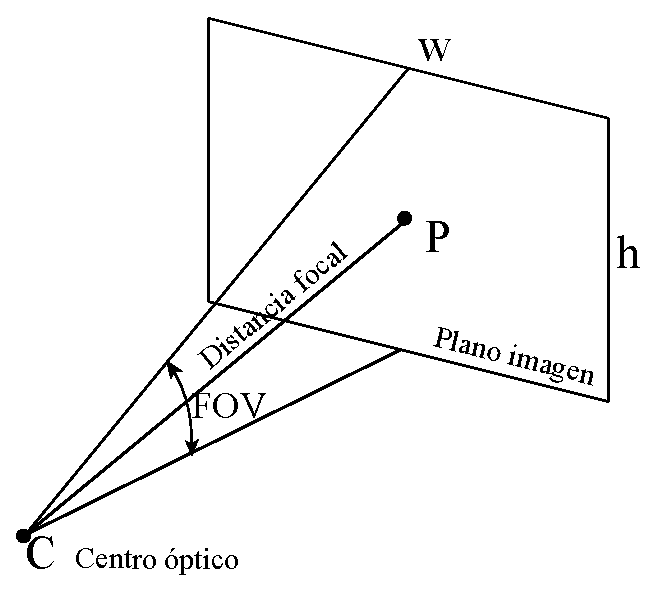
\includegraphics[scale=0.7]{figs_render/render1}
\caption{Definici�n gr�fica del FOV.}
\label{fig:render1}
\end{figure}

Realizando algo de geometr�a se ve que la relaci�n entre la distancia focal y el FOV es:
\[
FOV = 2.arctg\left(\frac{h}{2.f}\right)
\]
donde $h$ denota la altura del plano imagen y $f$ la distancia focal de la c�mara.\\

Otra particularidad de ISGL3D es el sistema de coordenadas que difiere del que se usa en algunas herramientas de modelado, como por ejemplo Blender, en las que el plano \textit{X-Y} se corresponde con el plano horizontal. Para ISGL3D los ejes est�n orientados como en la Figura \ref{fig:ejes}, con el origen en el centro del plano de la pantalla del dispositivo que coincide con el plano \textit{X-Y}, y el eje \textit{Z} saliente de la misma.\\	
\\
\begin{figure}[h!]
\centering
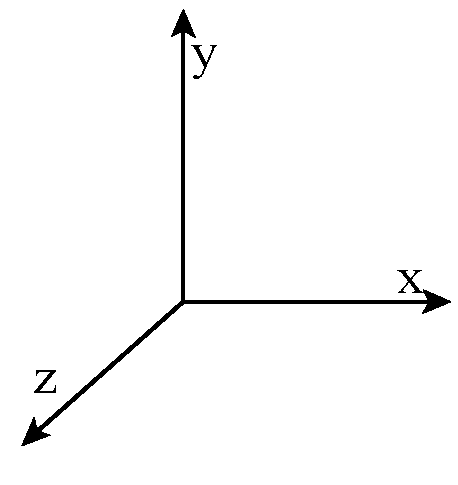
\includegraphics[scale=0.7]{figs_render/ejes.pdf}
\caption{Sistema de coordenadas de ISGL3D.}
\label{fig:ejes}
\end{figure}

\section{Primitivas de ISGL3D}
ISGL3D cuenta con algunas estructuras primitivas que pueden ser usadas como modelos, o incluso combinadas de manera de formar modelos algo m�s complejos. Las principales estructuras primitivas de ISGL3D son:
\begin{itemize}
\item \textbf{Isgl3DArrow:} modelo correspondiente a una flecha. Tiene 4 par�metros configurables:
\begin{itemize}
\item \textit{headHeight:} altura de la punta.
\item \textit{headRadius:} radio de la punta.
\item \textit{height:} altura total de la flecha.
\item \textit{radius:} radio de la base.
\end{itemize} 
\item \textbf{Isgl3DCone:} modelo correspondiente a un cono. Tiene 3 par�metros configurables:
\begin{itemize}
\item \textit{bottomRadius:} radio de la base inferior.
\item \textit{height:} altura del cono.
\item \textit{topRadius:} radio de la base superior.
\end{itemize}
\item \textbf{Isgl3DCube:} modelo correspondiente a un cubo. Tiene 3 par�metros configurables:
\begin{itemize}
\item \textit{depth:} profundidad del cubo. 
\item \textit{height:} altura del cubo.
\item \textit{width:} anchura del cubo.
\end{itemize}
\item \textbf{Isgl3DCylinder:} modelo correspondiente a un cilindro. Tiene 3 par�metros configurables:
\begin{itemize}
\item \textit{height:} altura del cilindio.
\item \textit{radius:} radio del cilindro.
\item \textit{openEnded:} indica si el cilindro cuenta con sus extremos abiertos o no.
\end{itemize}
\item \textbf{Isgl3DEllipsoid:} modelo correspondiente a una elipsoide. Cuenta con 3 par�metros configurables:
\begin{itemize}
\item \textit{radiusX:} radio de la elipsoide en la direcci�n \textit{x}.
\item \textit{radiusY:} radio de la elipsoide en la direcci�n \textit{y}.
\item \textit{radiusZ:} radio de la elipsoide en la direcci�n \textit{z}.
\end{itemize}
\item \textbf{Isgl3DOvoid:} modelo ovoide. Cuenta con 3 par�metros configurables:
\begin{itemize}
\item \textit{a:} radio del ovoide en la direcci�n \textit{x}. 
\item \textit{b:} radio del ovoide en la direcci�n \textit{y}.
\item \textit{k:} factor que modifica la forma de la curva. Cuando toma el valor 0, el modelo se corresponde con el de una ellipsoide.
\end{itemize}
\item \textbf{Isgl3DSphere:} modello correspondiente a una esfera. Tiene un �nico par�metro configurable:
\begin{itemize}
\item \textit{radius:} radio de la esfera.
\end{itemize}
\item \textbf{Isgl3DTorus:} modelo correspondiente a un toroide. Cuenta con 2 par�metros configurables:
\begin{itemize}
\item \textit{radius:} radio desde el origen del toroide hasta el centro del tubo.
\item \textit{tubeRadius:} radio del tubo del toroide.
\end{itemize}
\end{itemize}

\begin{figure}[h!]
\centering
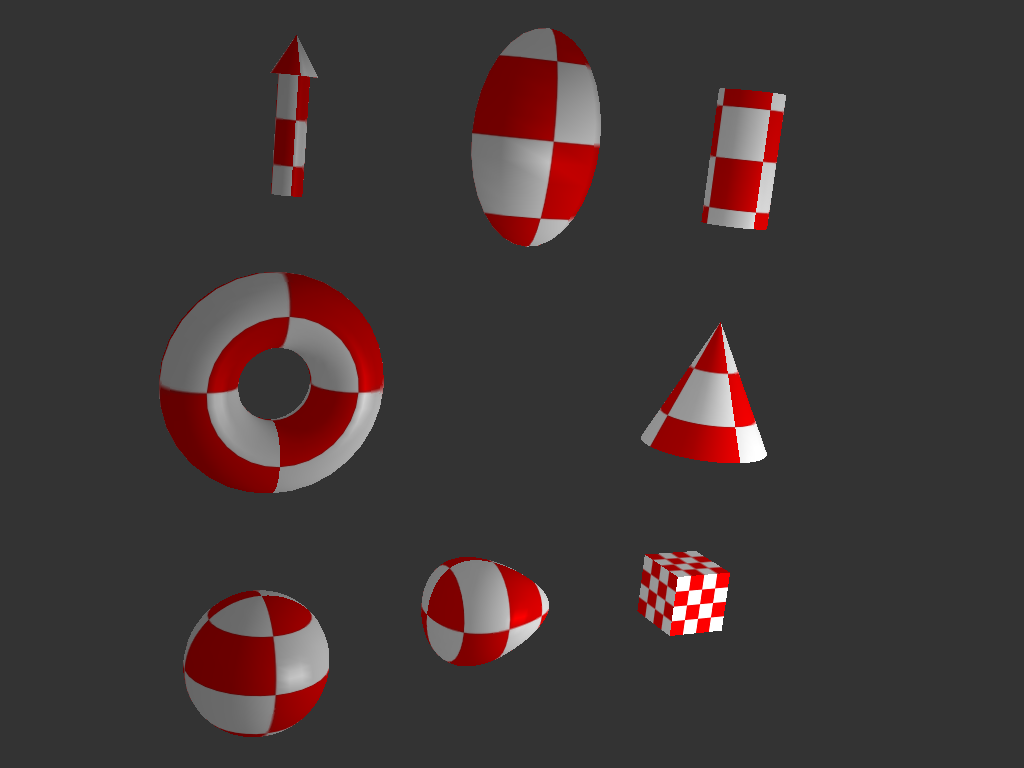
\includegraphics[scale=0.2]{figs_render/render2}
\caption{Principales primitivas en ISGL3D.}
\label{fig:render2}
\end{figure}

Para la creaci�n de cada primitiva, se debe especificar adem�s, la cantidad de segmentos que la forman en las distintas dimensiones. En la figura \ref{fig:render2} se pueden ver todas las primitivas anteriores. Es f�cil ver que dichas primitivas cuentan con cierta textura cuadriculada de colores rojo y blanco, que fue lograda mapeando una imagen sobre cada una de ellas. La porci�n de c�digo que se us� para realizar tal mapeo se muestra a continuaci�n:\\
\footnotesize
\begin{verbatim}
Isgl3dTextureMaterial * material = [Isgl3dTextureMaterial
                  materialWithTextureFile:@"red_checker.png" shininess:0.9];
	
Isgl3dTorus * torusMesh = [Isgl3dTorus meshWithGeometry:2 tubeRadius:1 ns:32 nt:32];

Isgl3dMeshNode * _torus = [self.scene createNodeWithMesh:torusMesh andMaterial:material];
\end{verbatim}

\normalsize
En la primera l�nea de c�digo se crea el material. Dicho material es del tipo \textit{Isgl3dTextureMaterial}; y la imagen con la que este se crea es la de la figura \ref{fig:render3}. Luego, se crea el toroide asign�ndole los par�metros vistos m�s atr�s en esta secci�n; y finalmente, se crea y se agrega a la escena el nodo asociado al toroide, con el material creado al principio. \\

\begin{figure}[h!]
\centering

\includegraphics[scale=0.5]{figs_render/red_checker}
\caption{Imagen \textit{red$\_$checker.png}, utilizada para crear la textura asociada a las primitivas de la figura \ref{fig:render2}.}
\label{fig:render3}
\end{figure}

\section{Importaci�n de modelos a ISGL3D.}
A veces lo que se quiere no es agregar a la escena una primitiva sino un modelo previamente creado. Los modelos son realizados en herramientas de creado y animaci�n de gr�ficos 3D como por ejemplo \textit{Blender}, \textit{MeshLab}, \textit{Autodesk Maya} o \textit{Autodesk 3ds Max}. Luego deben ser exportados en un formato llamado \textit{COLLADA}, acr�nimo de ``COLLAborative Design Activity'', que sirve para el intercambio de contenido digital 3D entre distintas aplicaciones de modelado. Por su parte, ISGL3D permite importar modelos pero en un formato llamado ``POD''. Se us� entonces, una aplicaci�n llamada \textit{Collada2POD} que lo que hace es convertir modelos tridimensionales en formato \textit{COLLADA} al formato POD. \textit{Collada2POD} puede ser descargada gratuitamente de la p�gina oficial de \textit{Imagination Technologies}, su desarrollador: \url{http://www.imgtec.com}. No esta de m�s aclarar que el proceso de conversi�n de formatos no es algo bueno; en ocasiones se vuelve problem�tico y puede resultar en un modelo que no anda como uno espera.\\

\begin{figure}[h!]
\centering
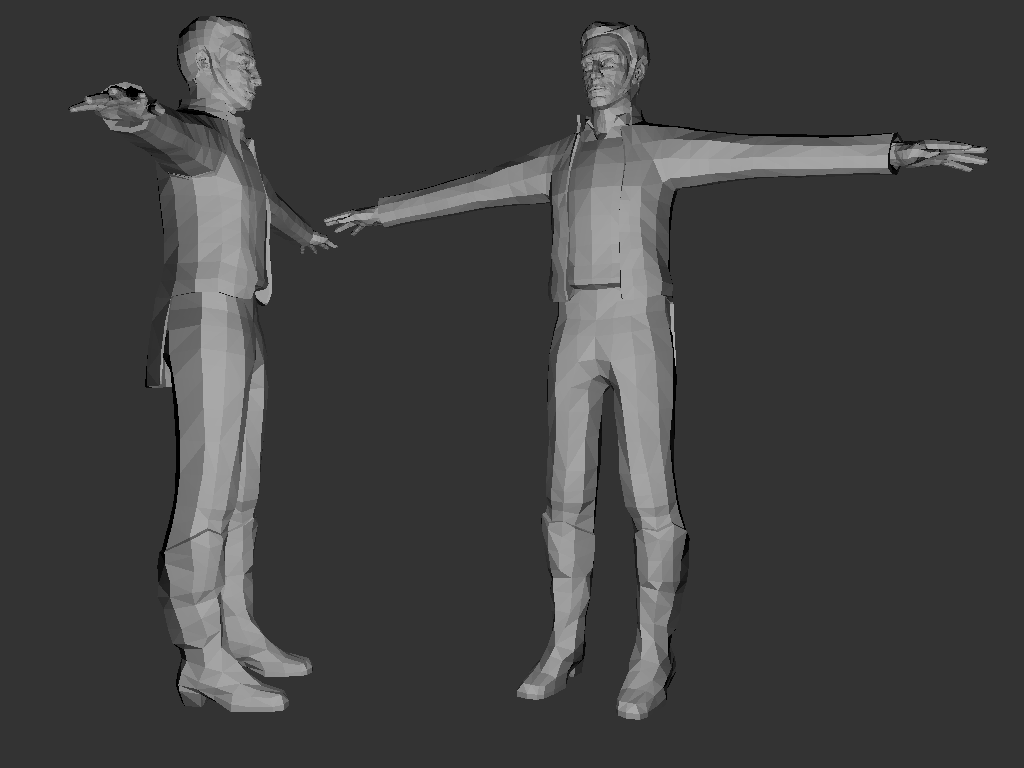
\includegraphics[scale=0.2]{figs_render/render4}
\caption{Modelo de Jos� Artigas agregado dos veces a una misma escena, pero visto desde �ngulos distintos.}
\label{fig:render4}
\end{figure}

Una vez que se tiene al objeto 3D en el formato requerido, este puede ser importado en ISGL3D de forma sencilla:\\
\footnotesize
\begin{verbatim}
Isgl3dPODImporter * podImporter = [Isgl3dPODImporter podImporterWithFile:@``modelo.pod''];

Isgl3dNode * _model = [self.scene createNode];

[podImporter addMeshesToScene:_model];

 _model.position = iv3(2, 6, 0);
\end{verbatim}

\normalsize
En la primera l�nea de c�digo se instancia la clase \textit{Isgl3dPODImporter} que sirve para transformar modelos POD a objetos ISGL3D, y se le asigna a la misma el modelo ``modelo.pod''. Luego, se crea un nodo llamado ``$\_$model'', al que se le asigna el modelo; y se agrega a la escena. Finalmente, se le asigna al nodo una posici�n. En la figura \ref{fig:render4} se puede ver un modelo de Jos� Artigas, agregado dos veces a una misma escena, pero visto desde �ngulos distintos.\\

Si lo que se quiere es que los modelos sean animados, o lo que es lo mismo, que tengan movimiento, hay dos soluciones posibles a tomar en consideraci�n:

\begin{itemize}
\item{\textbf{Modelo animado}}: muchas veces lo que se tiene es un modelo 3D animado desde su construcci�n. Estos pueden ser creados, al igual que los modelos 3D inanimados, con las herramientas para el creado y la animaci�n de gr�ficos 3D antedichas. Lo que se hace es agregarle al modelo un ``esqueleto'' que al moverlo, le transmite a dicho modelo su movimiento. Existe mucha bibliograf�a al respecto, adem�s de haber m�ltiples sitios en Internet de donde bajar los modelos, incluso en forma gratuita. Luego de obtenido el modelo animado, lo que se tiene es precisamente al modelo, pero con una l�nea de tiempo con las animaciones. Nuevamente, hay que convertirlo a formato POD para ser usado en ISGL3D. El c�digo para poder visualizar al modelo es:
\footnotesize
\begin{verbatim}
Isgl3dPODImporter * podImporter = [Isgl3dPODImporter 
             podImporterWithFile:@"animated_model.pod"];

Isgl3dSkeletonNode *_model = [self.scene createSkeletonNode];
   
[podImporter addMeshesToScene:_model];
   
Isgl3dAnimationController * _animationController = [[Isgl3dAnimationController alloc] 
            initWithSkeleton:_model andNumberOfFrames:[podImporter numberOfFrames]];
                                    
[_animationController start];
\end{verbatim}
\normalsize
En la primera l�nea de c�digo se instancia la clase \textit{Isgl3dPODImporter}, y se le asigna a la misma el modelo animado ``animated$\_$model.pod''.  Luego, se crea y se agrega a la escena un nodo del tipo \textit{Isgl3dSkeletonNode} llamado ``$\_$model'' que contiene al modelo animado. La clase \textit{Isgl3dSkeletonNode} provee una interfaz sencilla para animar al ahora objeto ISGL3D, que con la ayuda de la clase \textit{Isgl3dAnimationController}, logra automatizar el movimiento del mismo. Finalmente, se instancia y configura la clase \textit{Isgl3dAnimationController} y se le da inicio a la animaci�n en la �ltima l�nea.\\

\item\textbf{M�ltiples modelos inanimados:} otra forma de animar un modelo 3D es usando m�ltiples modelos inanimados. Estos pueden ser cargados en ISGL3D como un �nico objeto o nodo y mediante ciertas instrucciones sencillas, se le dice al \textit{framework} que presente uno a continuaci�n del otro, interpolando entre posiciones contiguas, lo que genera una sensaci�n de movimento. Este fue el m�todo utilizado en el presente proyecto para animar al modelo de Jos� Artigas. En la figura \ref{fig:render5} se puede ver al mismo en 3 posiciones distintas.\\

\begin{figure}[h!]
\centering
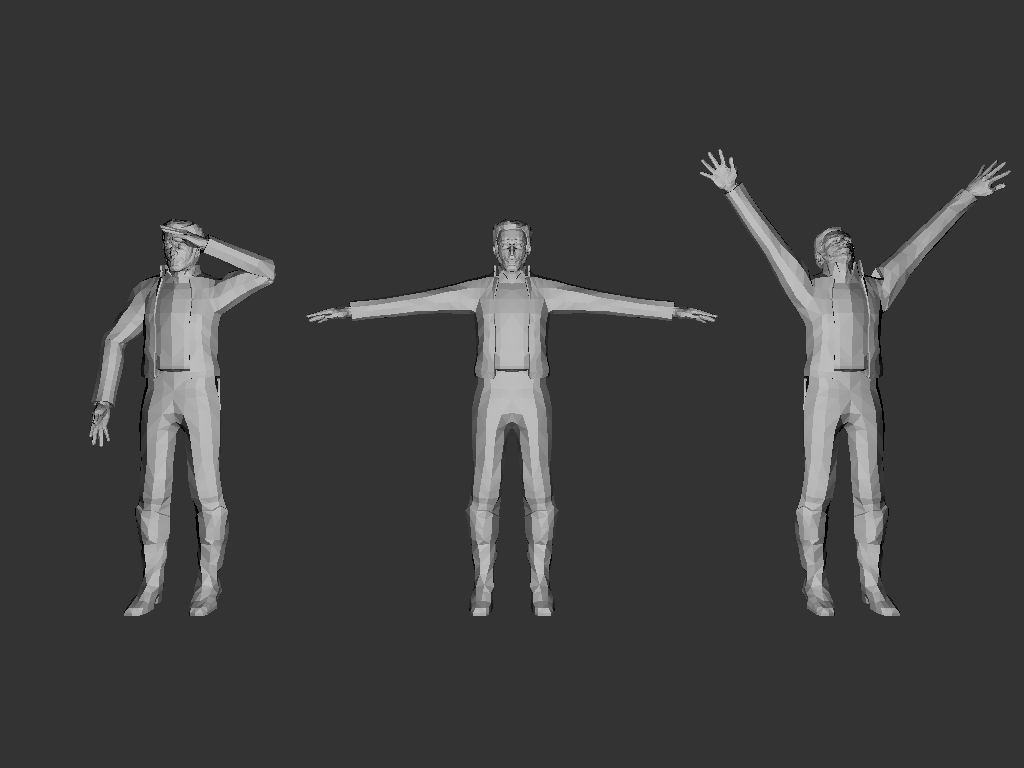
\includegraphics[scale=0.3]{figs_render/artigases}
\caption{Modelo de Jos� Artigas en 3 posiciones distintas, utilizadas  para generar en ISGL3D una sensaci�n de movimiento.}
\label{fig:render5}
\end{figure}

El c�digo para realizar la interpolaci�n mencionada, aplicado por ejemplo a dos modelos, ser�:
\footnotesize
\begin{verbatim}
Isgl3dPODImporter * podImporter = [Isgl3dPODImporter 
          podImporterWithFile:@"model_1.pod"];

[podImporter buildSceneObjects];
        
Isgl3dPODImporter * podImporter2 = [Isgl3dPODImporter 
         podImporterWithFile:@"model_2.pod"];

[podImporter2 buildSceneObjects];

Isgl3dGLMesh* _modelMesh = [podImporter meshAtIndex:0 ];
 
Isgl3dGLMesh* _modelMesh2 = [podImporter2 meshAtIndex:0 ];

Isgl3dKeyframeMesh * _mesh = [Isgl3dKeyframeMesh keyframeMeshWithMesh:_modelMesh];
          
[_mesh addKeyframeMesh:_modelMesh2];
        
[_mesh addKeyframeAnimationData:0 duration:1.0f];
[_mesh addKeyframeAnimationData:0 duration:2.0f];
[_mesh addKeyframeAnimationData:1 duration:1.0f];
[_mesh addKeyframeAnimationData:1 duration:2.0f];

[_mesh startAnimation];

Isgl3dNode * node = [_container createNodeWithMesh:_mesh 
          andMaterial:[podImporter materialWithName:@"material_0"]];

node.position = iv3(-90, -60, -150);

[podImporter addMeshesToScene:node];
\end{verbatim}
\normalsize
En las primeras 4 l�neas de c�digo se instancia en dos oportunidades la clase \textit{Isgl3dPODImporter}, y se les asigna a las instancias los modelos inanimados ``model$\_$1.pod'' y ``model$\_$2.pod'. La instrucci�n \textit{buildSceneObjects} crea todos los objetos de la escena del modelo POD, pero no los agrega a la escena ISGL3D. Luego se obtienen los modelos indexados de cada uno de los PODs (cada POD puede tener una escena con m�s de un modelo, mediante un �ndice se referencia qu� modelo se quiere obtener) y se almacenan en ``$\_$modelMesh'' y ``$\_$modelMesh2'' respectivamente. Se genera a continuaci�n un nuevo modelo al que se le asignan los dos modelos anteriores, luego se programa la animaci�n y se le da inicio mediante la instrucci�n \textit{startAnimation}. Finalmente, se genera un nuevo objeto o nodo ISGL3D al que se le asigna el modelo, y un material tambi�n cargado desde el archivo POD; se le asigna adem�s una posici�n y se lo agrega a la escena. 
\end{itemize}

\section{Luz en ISGL3D}
%http://isgl3d.com/tutorials/3/tutorial_2_lighting_and_shading
Un tema importante al momento de proyectar modelos 3D en una escena es la luz. La visualizaci�n de un modelo puede cambiar significativamente en funci�n de las caracter�sticas de luz que tenga una escena. En ISGL3D la luz se logra mediante la suma de tres componentes independientes: \textit{ambiente}, \textit{difusa} y \textit{especular}; siendo esto un est�ndar en todos los motores de juego y programas de modelado en general. La luz ambiente es no direccional y est� presente en toda la escena. La luz difusa ya implica la reacci�n que tiene la luz proveniente de las distintas fuentes de luz direccionales sobre las superficies de los objetos que existen en la escena generando haces de luz en direcciones aleatorias. La luz especular modela el comportamiento de la luz reflejada sobre las distintas superficies en ciertas direcciones particulares (no aleatorias) que dependen del coeficiente de reflexi�n de los materiales. Cada uno de estos tres tipos de luz que modelan el mundo real, existen en ISGL3D y son representados como caracter�sticas configurables de los objetos de luz. A su vez existen fuentes lum�nicas de distintos tipos: \textit{puntual}, \textit{direccional} y \textit{c�nica}. Cada tipo tiene una funci�n distinta de la  atenuaci�n con respecto a la distancia. Un ejemplo de la creaci�n de un elemento lum�nico para una escena se ve en el siguiente c�digo:

\begin{verbatim}
Isgl3dLight * _redLight = [Isgl3dLight lightWithHexColor:@"FF0000" diffuseColor:
@"FF0000" specularColor:@"FFFFFF" attenuation:0.02];
_redLight.renderLight = YES;
[self.scene addChild:_redLight];
\end{verbatim}

En la primera l\'inea de c\'odigo se crea una luz con una componente ambiente de color rojo, una componente difusa tambi�n de color rojo y una componente especular de color blanca. En todos los casos se usa la notaci�n hexadecimal de las componentes RGBA. Adem�s se escogi� un valor $0,02$ de atenuaci\'on. Luego, se pide que el foco de luz s\'i sea \textit{renderizado} y finalmente, este es agregado a la escena. Por defecto, el tipo de luz utilizado es puntual.

\section{M�todo \textit{- (void) tick:(float)dt}}
Cuando se instancia la clase encargada de generar el render (clase \textit{HelloWorldView}), la misma ejecuta la configuraci�n b�sica de inicializaci�n del objeto. Entre otras cosas, dentro del c�digo de inicializaci�n, se agrega lo siguiente:

\begin{verbatim}
[self schedule:@selector(tick:)];
\end{verbatim}

Esto lo que hace es ``agendarse'' una invocaci�n del m�todo \textit{tick} en forma peri�dica. Dentro de dicho m�todo es que se hace la actualizaci�n de la escena, y el en caso particular de este proyecto, es en d�nde se actualiza la posici�n de los objetos 3D en funci�n de la posici�n de la c�mara respecto de los ejes del mundo. Ver Cap�tulo \ref{chap: camypose}. Este m�todo es de vital importancia por tratarse de uno de los dos \textit{callbacks} que toda aplicaci�n de realidad aumentada tiene (el otro es la captura y procesamiento de la imagen para obtener la pose).

\section{ISGL3D en la aplicaci�n}
En el Cap�tulo \ref{chap: imp} se explican algunos detalles sobre el uso de ISGL3D dentro de la aplicaci�n final. En particular se dan detalles constructivos sobre c�mo utilizar esta herramienta para generar \textit{renders} sobre un fondo que sea la captura de la c�mara y de la convivencia de los dos \textit{callbacks} de la aplicaci�n.

\section{Resumen}

En el presente cap\'itulo se mencionaron algunas herramientas existentes para realizar \textit{renders} en dispositivos m\'oviles con sistema operativo iOS. Luego, se justific\'o la elecci\'on de ISGL3D para tal funci\'on y se dieron algunos conceptos introductorios a la herramienta; adem\'as se di\'o una hoja de ruta para todo aquel que le interese ampliar sus conocimientos en el \textit{framework}. Se indicaron dos formas distintas de embeber un modelo 3D en ISGL3D y se aclar\'o cu\'al fue la forma escogida por el grupo. Finalmente, se referenci\'o el Cap\'itulo \ref{chap: imp}, en donde se explica c�mo se us� ISGL3D en la aplicaci�n final. 




\bibliographystyle{unsrt}   
\bibliography{encuadro}  
\end{document}
